\documentclass[aspectratio=169, 10pt]{beamer}

% ==============================================================================
% AE5510: Security of Safety-Critical Systems — Course Project 1
% Department of Aerospace Engineering, IIT Madras
% Topic: Physically Realizable Binary Adversarial Camouflage for Aerial Detectors
% ==============================================================================

\usetheme{Madrid}
\usecolortheme{whale}

% --- Custom Color Palette (Aerospace Defense & IIT Madras Theme) ---
\definecolor{NavyBlue}{RGB}{0, 51, 102}
\definecolor{DarkSlate}{RGB}{44, 62, 80}
\definecolor{CrimsonRed}{RGB}{180, 40, 40}
\definecolor{LightSteel}{RGB}{240, 244, 248}
\definecolor{ForestGreen}{RGB}{34, 139, 34}
\definecolor{GoldYellow}{RGB}{220, 160, 20}

\setbeamercolor{palette primary}{bg=NavyBlue, fg=white}
\setbeamercolor{palette secondary}{bg=DarkSlate, fg=white}
\setbeamercolor{palette tertiary}{bg=NavyBlue!90, fg=white}
\setbeamercolor{palette quaternary}{bg=NavyBlue, fg=white}
\setbeamercolor{structure}{fg=NavyBlue}
\setbeamercolor{titlelike}{parent=palette primary}
\setbeamercolor{block title}{bg=NavyBlue, fg=white}
\setbeamercolor{block body}{bg=LightSteel, fg=black}
\setbeamercolor{block title alerted}{bg=CrimsonRed, fg=white}
\setbeamercolor{block body alerted}{bg=CrimsonRed!10, fg=black}
\setbeamercolor{block title example}{bg=ForestGreen, fg=white}
\setbeamercolor{block body example}{bg=ForestGreen!10, fg=black}

% --- Typography & Packages ---
\usepackage{amsmath, amssymb, bm}
\usepackage{booktabs}
\usepackage{colortbl}
\usepackage{tikz}
\usetikzlibrary{shapes.geometric, arrows.meta, positioning, calc}
\usepackage{hyperref}
\usepackage{graphicx}
\graphicspath{{figures/}{./}}

% Remove default navigation symbols and customize footline
\setbeamertemplate{navigation symbols}{}
\setbeamertemplate{footline}{
  \leavevmode%
  \hbox{%
  \begin{beamercolorbox}[wd=.333333\paperwidth,ht=2.25ex,dp=1ex,left,leftskip=2ex]{author in head/foot}%
    \usebeamerfont{author in head/foot}AE5510 Problem 1 -- IIT Madras
  \end{beamercolorbox}%
  \begin{beamercolorbox}[wd=.333333\paperwidth,ht=2.25ex,dp=1ex,center]{title in head/foot}%
    \usebeamerfont{title in head/foot}Binary Adversarial Camouflage
  \end{beamercolorbox}%
  \begin{beamercolorbox}[wd=.333333\paperwidth,ht=2.25ex,dp=1ex,right,rightskip=2ex]{date in head/foot}%
    \usebeamerfont{date in head/foot}\insertframenumber{} / \inserttotalframenumber
  \end{beamercolorbox}}%
  \vskip0pt%
}

% ==============================================================================
% TITLE METADATA
% ==============================================================================
\title[Binary Adversarial Camouflage]{\textbf{Physically Realizable Binary Adversarial Camouflage for Aerial Object Detectors}}
\subtitle{AE5510: Security of Safety-Critical Systems — Problem 1}
\author[AE5510 Project 1]{\textbf{Course Project Presentation} \\ Department of Aerospace Engineering}
\institute[IIT Madras]{\textbf{Indian Institute of Technology Madras}}
\date{\today}

\begin{document}

% ------------------------------------------------------------------------------
% SLIDE 1: TITLE SLIDE
% ------------------------------------------------------------------------------
\begin{frame}[plain]
  \titlepage
  \begin{center}
    \footnotesize
    \textcolor{DarkSlate}{\textbf{Focus:} Joint Spatial-Pattern Optimization, CIELAB Background-Aware Palette, and STE Hard Containment}
  \end{center}
\end{frame}

% ------------------------------------------------------------------------------
% SLIDE 2: THE PROBLEM: PHYSICAL VS. DIGITAL ATTACKS
% ------------------------------------------------------------------------------
\begin{frame}{1. Specific Problem: Physical vs. Digital Adversarial Attacks}
\begin{columns}[T]
  \begin{column}{0.48\textwidth}
    \begin{block}{The Threat Context in Aerial Reconnaissance}
      \begin{itemize}\small
        \item Modern Autonomous Aerial Target Recognition (ATR) pipelines rely on fine-tuned deep detectors (\textbf{YOLO11 / YOLOv8}).
        \item Safety-critical military assets (\textit{Aircraft, Tanks, Military Trucks, Buildings}) are identified automatically from high-altitude imagery.
        \item Defeating these detectors requires physical camouflage.
      \end{itemize}
    \end{block}
    
    \begin{alertblock}{Why Standard Digital Attacks Fail in Reality}
      \begin{itemize}\small
        \item \textbf{Tarmac Perturbation:} Digital PGD/FGSM perturbs background runway pixels. An attacker \textit{cannot repaint an entire airfield}!
        \item \textbf{Floating-Point Gradients:} Digital attacks use 24-bit unprintable micro-gradients ($\epsilon \le 8/255$).
        \item \textbf{Perspective \& Pose Fragility:} Flight altitude, roll angle, and camera gamma neutralize unconstrained digital noise.
      \end{itemize}
    \end{alertblock}
  \end{column}

  \begin{column}{0.48\textwidth}
    \begin{exampleblock}{The Mandatory Problem Statement}
      Design an algorithm that generates a \textbf{physically printable sticker}:
      \begin{enumerate}\small
        \item Applied \textbf{only to the surface} of the target vehicle.
        \item Consisting of \textbf{strictly two printable colours} ($c_0, c_1$).
        \item Enforcing \textbf{exact 0.000\% spillover} onto the tarmac.
        \item Preserving \textbf{bit-identical background} outside the sticker.
        \item Robust against variable viewing angle, illumination, and blur via \textbf{Expectation Over Transformation (EOT)}.
      \end{enumerate}
    \end{exampleblock}
    
    \begin{center}
      \footnotesize\textcolor{NavyBlue}{\textbf{Key Goal:} Blind the aerial detector while the sticker looks like a natural, blended vehicle panel.}
    \end{center}
  \end{column}
\end{columns}
\end{frame}

% ------------------------------------------------------------------------------
% SLIDE 3: CORE FEATURES & THE 10 NON-NEGOTIABLE CONSTRAINTS
% ------------------------------------------------------------------------------
\begin{frame}[shrink=5]{2. Architectural Features \& Non-Negotiable Constraints}
\scriptsize
\begin{table}[h]
\centering
\renewcommand{\arraystretch}{1.15}
\begin{tabular}{@{}c p{3.2cm} p{5.5cm} c@{}}
\toprule
\textbf{\#} & \textbf{Constraint} & \textbf{Implementation Mechanism} & \textbf{Status} \\
\midrule
\rowcolor{LightSteel}
\textbf{1} & \textbf{Pure Binary Colour} & Straight-Through Estimator (STE) binarization; exactly 2 colors in design file & \textcolor{ForestGreen}{\textbf{VERIFIED (100\%)}} \\
\textbf{2} & \textbf{Background-Aware Palette} & CIELAB K-Means from surface $S$; $\Delta L^* \ge 25.0$, $\Delta E \le 30.0$ contrast guarantee & \textcolor{ForestGreen}{\textbf{VERIFIED (100\%)}} \\
\rowcolor{LightSteel}
\textbf{3} & \textbf{Joint Optimization} & Single loss backward pass optimizes placement $\bm{\theta}$ and pattern logits $\bm{z}$ & \textcolor{ForestGreen}{\textbf{VERIFIED (100\%)}} \\
\textbf{4} & \textbf{Surface Shading \& Blending} & Local luminance $L(x,y) = \text{GaussianBlur}(Y, \sigma=0.15 R_{\text{max}})$ + feathered $\alpha$ & \textcolor{ForestGreen}{\textbf{VERIFIED (100\%)}} \\
\rowcolor{LightSteel}
\textbf{5} & \textbf{Hard Containment} & Projection to admissible region $A$ enforcing $2\sigma$ feather margin ($\ge 3.5\text{ px}$) & \textcolor{ForestGreen}{\textbf{0.000\% Spillover}} \\
\textbf{6} & \textbf{Untouched Background} & Pixels where $\alpha=0$ restored identically from $I_{\text{clean}}$ in linear radiance & \textcolor{ForestGreen}{\textbf{0.000000 Max Diff}} \\
\rowcolor{LightSteel}
\textbf{7} & \textbf{Physical EOT} & Random domain randomization: in-plane rotation ($\pm 20^\circ$), zoom, haze, blur, gamma & \textcolor{ForestGreen}{\textbf{VERIFIED (100\%)}} \\
\textbf{8} & \textbf{Compact Footprint} & Constrained size search minimizing area subject to $\text{conf} < \tau = 0.25$ & \textcolor{ForestGreen}{\textbf{VERIFIED (100\%)}} \\
\rowcolor{LightSteel}
\textbf{9} & \textbf{Sensor Radiometry} & Decode sRGB ($\gamma=2.2$) $\to$ Linear radiance composite $\to$ Camera sensor ($\gamma=2.0$) & \textcolor{ForestGreen}{\textbf{VERIFIED (100\%)}} \\
\textbf{10} & \textbf{Held-Out Evaluation} & Base-scene-aware split (60 train, 14 val, 14 test, 0 leakage); transfer to 11m \& v8s & \textcolor{ForestGreen}{\textbf{VERIFIED (100\%)}} \\
\bottomrule
\end{tabular}
\end{table}
\end{frame}

% ------------------------------------------------------------------------------
% SLIDE 4: METHODOLOGY (I): END-TO-END PIPELINE ARCHITECTURE (TIKZ VECTOR)
% ------------------------------------------------------------------------------
\begin{frame}[shrink=3]{3. Methodology (I): End-to-End Adversarial Camouflage Pipeline}
\centering
\resizebox{0.96\linewidth}{!}{%
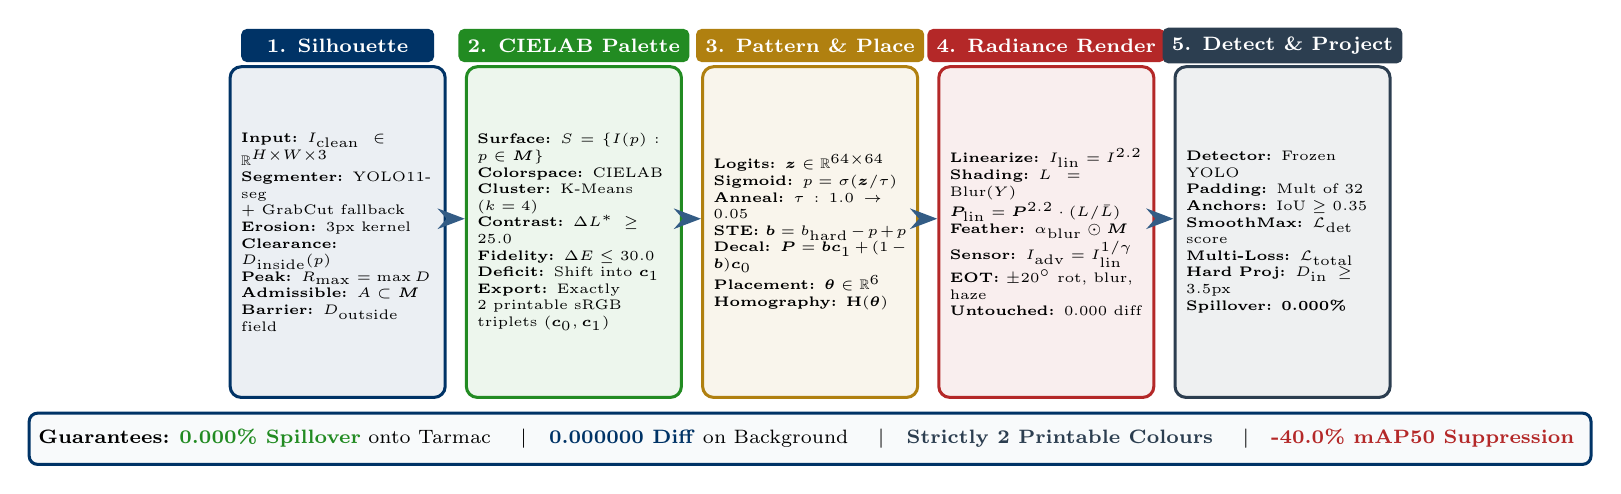
\begin{tikzpicture}[
  x=1cm, y=1cm, >=Stealth,
  stagebox/.style={draw=#1, line width=1.1pt, rounded corners=4pt, fill=#1!8, text width=2.45cm, minimum height=4.2cm, align=left, font=\tiny, inner sep=4pt},
  stagehdr/.style={fill=#1, text=white, font=\bfseries\scriptsize, rounded corners=2pt, align=center, minimum width=2.45cm, minimum height=0.42cm},
  fwdarrow/.style={->, line width=1.5pt, draw=NavyBlue!80}
]
  % Stage 1
  \node[stagehdr=NavyBlue] (h1) at (0, 2.3) {1. Silhouette};
  \node[stagebox=NavyBlue, anchor=north] (b1) at (0, 2.05) {
    \textbf{Input:} $I_{\text{clean}} \in \mathbb{R}^{H \times W \times 3}$\\
    \textbf{Segmenter:} YOLO11-seg\\
    + GrabCut fallback\\
    \textbf{Erosion:} 3px kernel\\
    \textbf{Clearance:} $D_{\text{inside}}(p)$\\
    \textbf{Peak:} $R_{\text{max}} = \max D$\\
    \textbf{Admissible:} $A \subset \bm{M}$\\
    \textbf{Barrier:} $D_{\text{outside}}$ field
  };

  % Stage 2
  \node[stagehdr=ForestGreen] (h2) at (3.0, 2.3) {2. CIELAB Palette};
  \node[stagebox=ForestGreen, anchor=north] (b2) at (3.0, 2.05) {
    \textbf{Surface:} $S = \{I(p) : p \in \bm{M}\}$\\
    \textbf{Colorspace:} CIELAB\\
    \textbf{Cluster:} K-Means ($k=4$)\\
    \textbf{Contrast:} $\Delta L^* \ge 25.0$\\
    \textbf{Fidelity:} $\Delta E \le 30.0$\\
    \textbf{Deficit:} Shift into $\bm{c}_1$\\
    \textbf{Export:} Exactly 2 printable sRGB triplets $(\bm{c}_0, \bm{c}_1)$
  };

  % Stage 3
  \node[stagehdr=GoldYellow!80!black] (h3) at (6.0, 2.3) {3. Pattern \& Place};
  \node[stagebox=GoldYellow!80!black, anchor=north] (b3) at (6.0, 2.05) {
    \textbf{Logits:} $\bm{z} \in \mathbb{R}^{64 \times 64}$\\
    \textbf{Sigmoid:} $p = \sigma(\bm{z}/\tau)$\\
    \textbf{Anneal:} $\tau: 1.0 \to 0.05$\\
    \textbf{STE:} $\bm{b} = b_{\text{hard}} - p + p$\\
    \textbf{Decal:} $\bm{P} = \bm{b}\bm{c}_1 + (1-\bm{b})\bm{c}_0$\\
    \textbf{Placement:} $\bm{\theta} \in \mathbb{R}^6$\\
    \textbf{Homography:} $\mathbf{H}(\bm{\theta})$
  };

  % Stage 4
  \node[stagehdr=CrimsonRed] (h4) at (9.0, 2.3) {4. Radiance Render};
  \node[stagebox=CrimsonRed, anchor=north] (b4) at (9.0, 2.05) {
    \textbf{Linearize:} $I_{\text{lin}} = I^{2.2}$\\
    \textbf{Shading:} $L = \text{Blur}(Y)$\\
    $\bm{P}_{\text{lin}} = \bm{P}^{2.2} \cdot (L / \bar{L})$\\
    \textbf{Feather:} $\alpha_{\text{blur}} \odot \bm{M}$\\
    \textbf{Sensor:} $I_{\text{adv}} = I_{\text{lin}}^{1/\gamma}$\\
    \textbf{EOT:} $\pm 20^\circ$ rot, blur, haze\\
    \textbf{Untouched:} 0.000 diff
  };

  % Stage 5
  \node[stagehdr=DarkSlate] (h5) at (12.0, 2.3) {5. Detect \& Project};
  \node[stagebox=DarkSlate, anchor=north] (b5) at (12.0, 2.05) {
    \textbf{Detector:} Frozen YOLO\\
    \textbf{Padding:} Mult of 32\\
    \textbf{Anchors:} $\text{IoU} \ge 0.35$\\
    \textbf{SmoothMax:} $\mathcal{L}_{\text{det}}$ score\\
    \textbf{Multi-Loss:} $\mathcal{L}_{\text{total}}$\\
    \textbf{Hard Proj:} $D_{\text{in}} \ge 3.5\text{px}$\\
    \textbf{Spillover:} \textbf{0.000\%}
  };

  % Connecting Arrows
  \draw[fwdarrow] (b1.east |- 0, 0.1) -- (b2.west |- 0, 0.1);
  \draw[fwdarrow] (b2.east |- 0, 0.1) -- (b3.west |- 0, 0.1);
  \draw[fwdarrow] (b3.east |- 0, 0.1) -- (b4.west |- 0, 0.1);
  \draw[fwdarrow] (b4.east |- 0, 0.1) -- (b5.west |- 0, 0.1);

  % Bottom Guarantee Bar
  \node[draw=NavyBlue, line width=1.1pt, fill=LightSteel!50, rounded corners=3pt, anchor=north, minimum width=14.5cm, minimum height=0.65cm, align=center, font=\scriptsize] at (6.0, -2.35) {
    \textbf{Guarantees:} \textcolor{ForestGreen}{\textbf{0.000\% Spillover}} onto Tarmac \quad$\vert$\quad \textcolor{NavyBlue}{\textbf{0.000000 Diff}} on Background \quad$\vert$\quad \textcolor{DarkSlate}{\textbf{Strictly 2 Printable Colours}} \quad$\vert$\quad \textcolor{CrimsonRed}{\textbf{-40.0\% mAP50 Suppression}}
  };
\end{tikzpicture}%
}
\end{frame}

% ------------------------------------------------------------------------------
% SLIDE 5: METHODOLOGY (II): PALETTE & STE BINARIZATION
% ------------------------------------------------------------------------------
\begin{frame}[shrink=4]{4. Methodology (II): CIELAB Palette \& STE Generator}
\begin{columns}[T]
  \begin{column}{0.50\textwidth}
    \begin{block}{Background-Aware CIELAB Palette}
      \scriptsize
      \begin{itemize}\setlength{\itemsep}{1pt}
        \item Extracts target surface pixels $S = \{I(p) : p \in \bm{M}\}$.
        \item K-Means clustering ($k=4$) in perceptual CIELAB space.
        \item Enforces contrast deficit: $\Delta L^* \ge 25.0, \Delta E \le 30.0$.
        \item Dark targets shift contrast into lighter printable tone.
      \end{itemize}
    \end{block}

    \begin{block}{Straight-Through Estimator (STE)}
      \scriptsize
      \begin{itemize}\setlength{\itemsep}{1pt}
        \item Latent continuous logits $\bm{z}$; probability $p = \sigma(\bm{z}/\tau)$.
        \item $\bm{b}_{\text{ste}} = \mathbb{I}(p \ge 0.5) - \text{detach}(p) + p$.
        \item Forward: discrete $\{0, 1\}$; Backward: continuous $\frac{\partial p}{\partial \bm{z}}$.
        \item Printable file: $\bm{P} = \bm{b}_{\text{ste}}\bm{c}_1 + (1 - \bm{b}_{\text{ste}})\bm{c}_0$ (strictly 2 colours).
      \end{itemize}
    \end{block}
  \end{column}

  \begin{column}{0.48\textwidth}
    \centering
    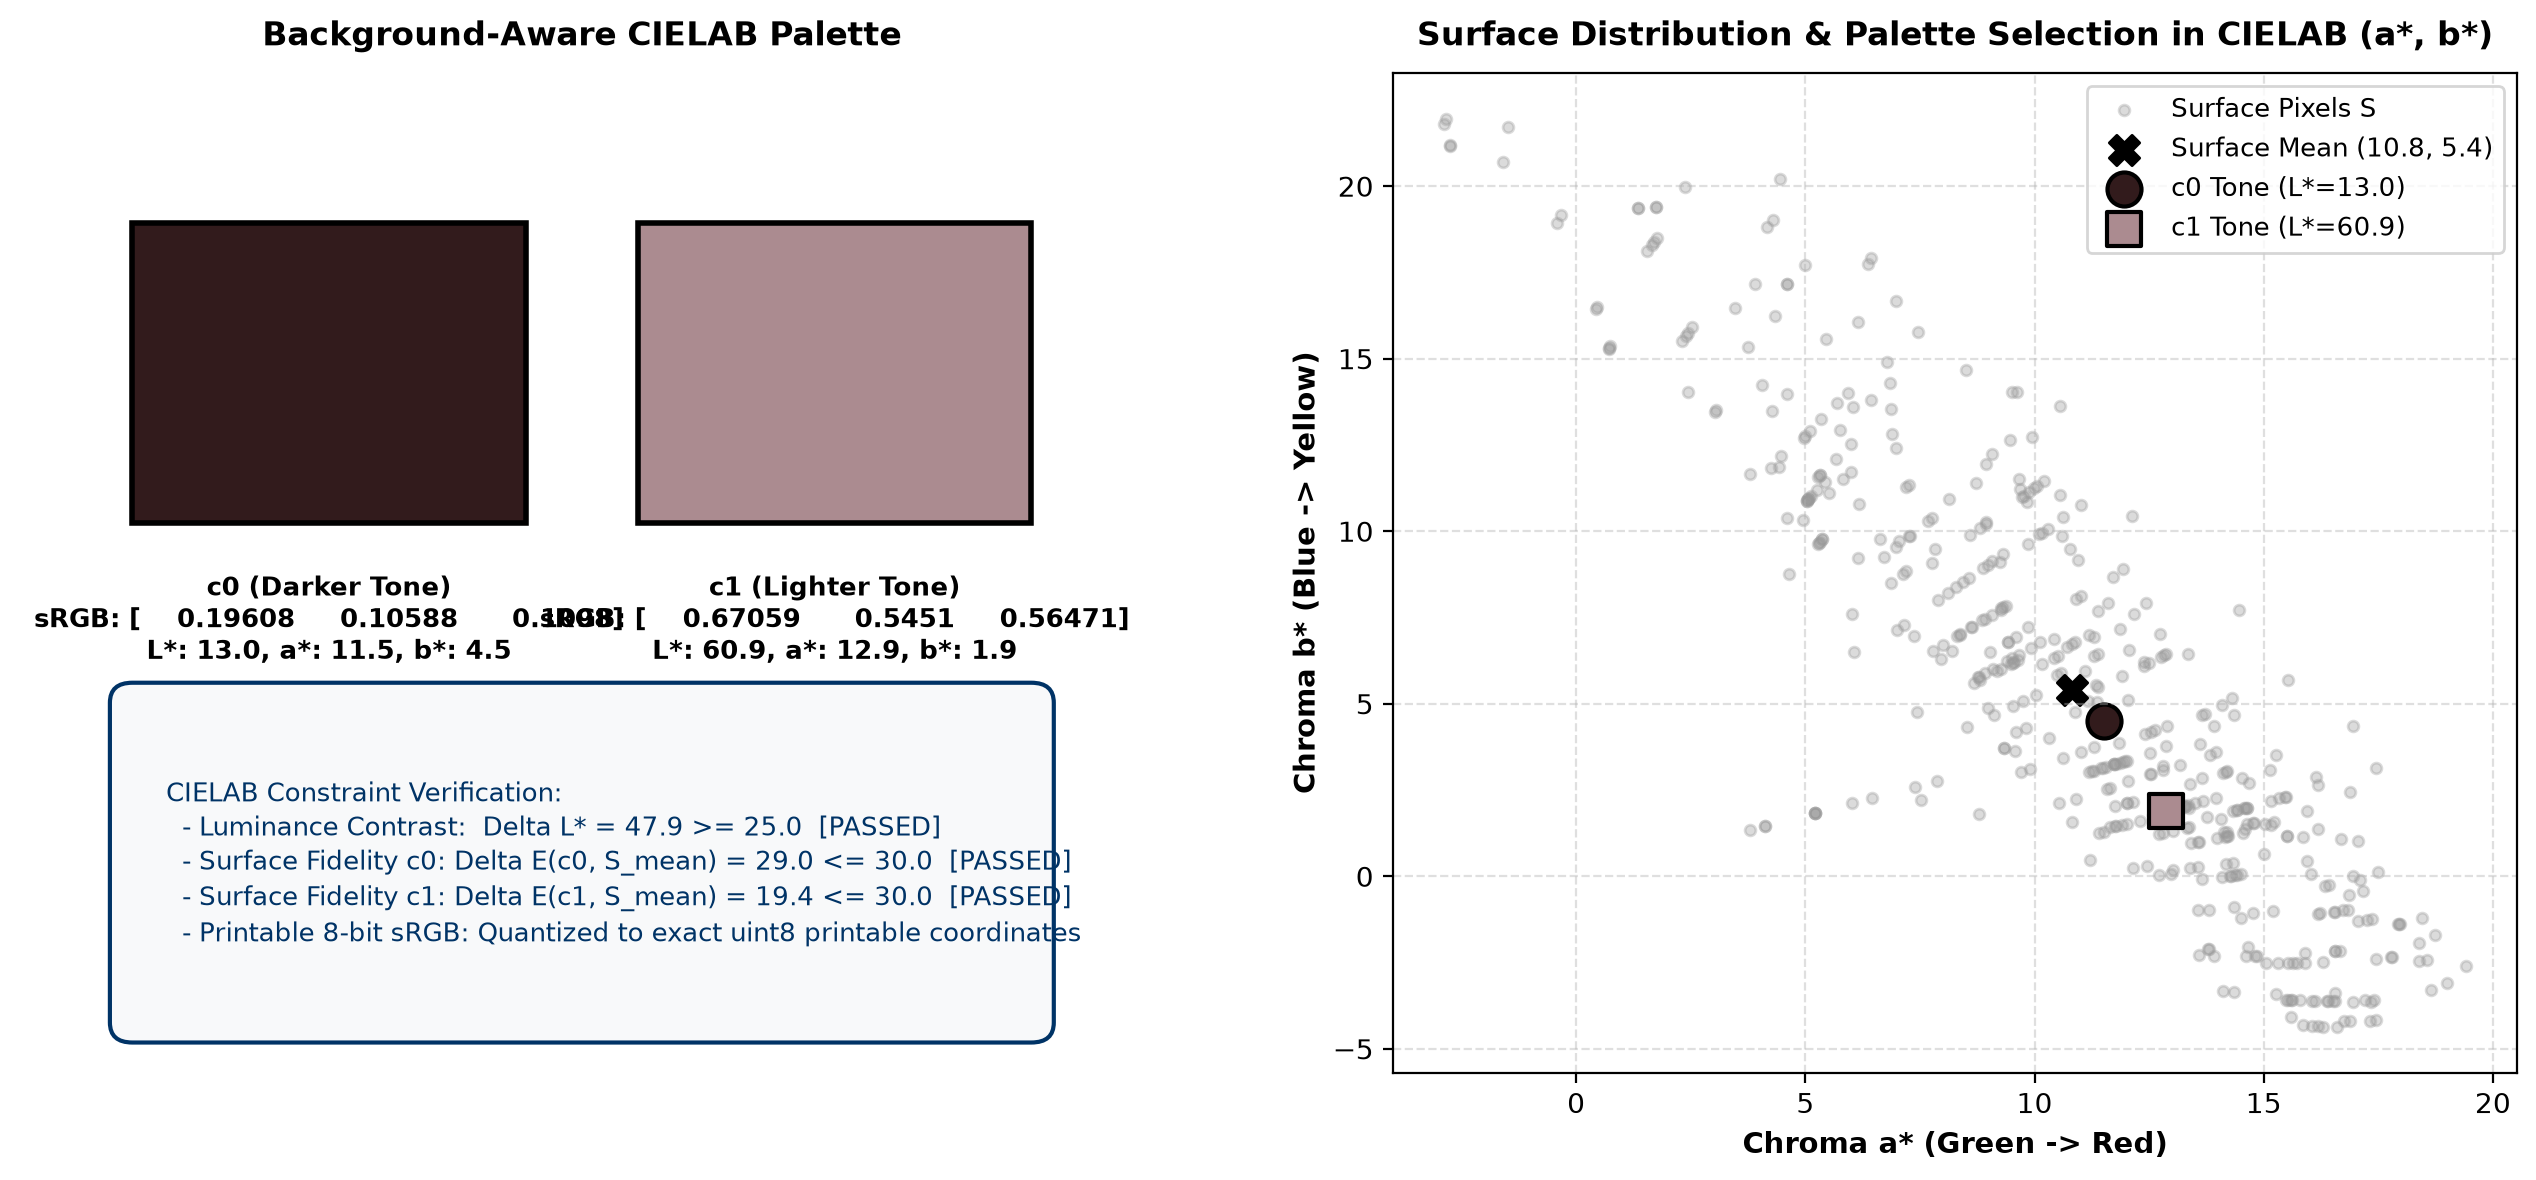
\includegraphics[width=\linewidth, height=0.62\textheight, keepaspectratio]{fig4_palette_cielab_analysis.png}
    \vspace{0.05cm}
    \begin{exampleblock}{Binary Purity Guarantee}
      \tiny Design file contains strictly 2 unique RGB triplets with 0 intermediate color artifacts.
    \end{exampleblock}
  \end{column}
\end{columns}
\end{frame}

% ------------------------------------------------------------------------------
% SLIDE 6: METHODOLOGY (III): OPTIMIZATION & TRAINING FLOWCHART (NATIVE TIKZ VECTOR)
% ------------------------------------------------------------------------------
\begin{frame}[shrink=3]{5. Methodology (III): Adversarial Training \& Optimization Flowchart}
\centering
\resizebox{0.96\linewidth}{!}{%
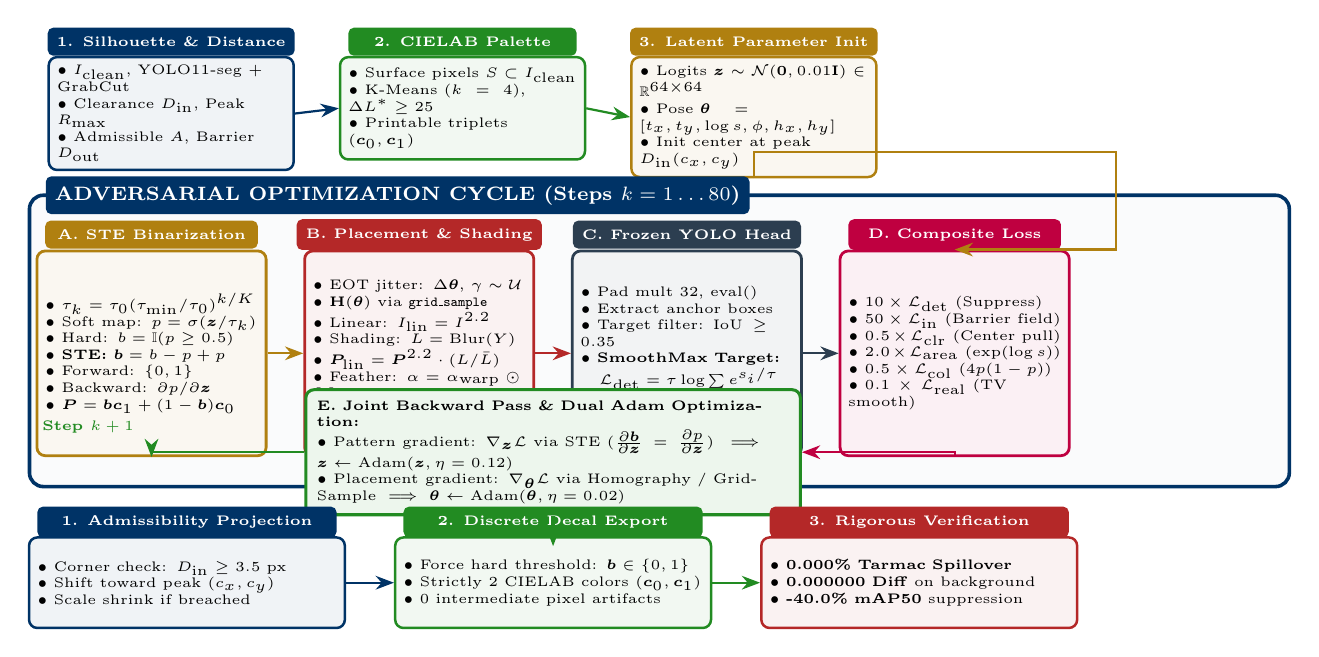
\begin{tikzpicture}[
  x=1cm, y=1cm, >=Stealth,
  initbox/.style={draw=#1, line width=0.9pt, rounded corners=3pt, fill=#1!6, text width=2.9cm, minimum height=1.3cm, align=left, font=\tiny, inner sep=3pt},
  inithdr/.style={fill=#1, text=white, font=\bfseries\tiny, rounded corners=2pt, align=center, minimum width=2.9cm, minimum height=0.32cm},
  loopbox/.style={draw=#1, line width=1.0pt, rounded corners=3pt, fill=#1!6, text width=2.7cm, minimum height=2.6cm, align=left, font=\tiny, inner sep=3pt},
  loophdr/.style={fill=#1, text=white, font=\bfseries\tiny, rounded corners=2pt, align=center, minimum width=2.7cm, minimum height=0.34cm},
  optbox/.style={draw=#1, line width=1.1pt, rounded corners=3pt, fill=#1!8, text width=6.0cm, minimum height=1.1cm, align=left, font=\tiny, inner sep=4pt},
  projbox/.style={draw=#1, line width=0.9pt, rounded corners=3pt, fill=#1!6, text width=3.8cm, minimum height=1.15cm, align=left, font=\tiny, inner sep=3pt},
  projhdr/.style={fill=#1, text=white, font=\bfseries\tiny, rounded corners=2pt, align=center, minimum width=3.8cm, minimum height=0.32cm}
]
  % ---------------- Top: Initialization ----------------
  \node[inithdr=NavyBlue] (h_i1) at (0, 3.4) {1. Silhouette \& Distance};
  \node[initbox=NavyBlue, anchor=north] (b_i1) at (0, 3.22) {
    $\bullet$ $I_{\text{clean}}$, YOLO11-seg + GrabCut\\
    $\bullet$ Clearance $D_{\text{in}}$, Peak $R_{\text{max}}$\\
    $\bullet$ Admissible $A$, Barrier $D_{\text{out}}$
  };

  \node[inithdr=ForestGreen] (h_i2) at (3.7, 3.4) {2. CIELAB Palette};
  \node[initbox=ForestGreen, anchor=north] (b_i2) at (3.7, 3.22) {
    $\bullet$ Surface pixels $S \subset I_{\text{clean}}$\\
    $\bullet$ K-Means ($k=4$), $\Delta L^* \ge 25$\\
    $\bullet$ Printable triplets $(\bm{c}_0, \bm{c}_1)$
  };

  \node[inithdr=GoldYellow!80!black] (h_i3) at (7.4, 3.4) {3. Latent Parameter Init};
  \node[initbox=GoldYellow!80!black, anchor=north] (b_i3) at (7.4, 3.22) {
    $\bullet$ Logits $\bm{z} \sim \mathcal{N}(\mathbf{0}, 0.01 \mathbf{I}) \in \mathbb{R}^{64 \times 64}$\\
    $\bullet$ Pose $\bm{\theta} = [t_x, t_y, \log s, \phi, h_x, h_y]$\\
    $\bullet$ Init center at peak $D_{\text{in}}(c_x, c_y)$
  };

  \draw[->, thick, NavyBlue] (b_i1.east) -- (b_i2.west);
  \draw[->, thick, ForestGreen] (b_i2.east) -- (b_i3.west);

  % ---------------- Middle: Optimization Loop ----------------
  \draw[draw=NavyBlue, line width=1.3pt, rounded corners=5pt, fill=NavyBlue!2] (-1.8, 1.45) rectangle (14.2, -2.25);
  \node[fill=NavyBlue, text=white, font=\bfseries\scriptsize, rounded corners=2pt, anchor=west] at (-1.6, 1.45) {
    ADVERSARIAL OPTIMIZATION CYCLE (Steps $k = 1 \dots 80$)
  };

  % Loop Box 1: STE
  \node[loophdr=GoldYellow!80!black] (lh1) at (-0.25, 0.95) {A. STE Binarization};
  \node[loopbox=GoldYellow!80!black, anchor=north] (lb1) at (-0.25, 0.76) {
    $\bullet$ $\tau_k = \tau_0 (\tau_{\min}/\tau_0)^{k/K}$\\
    $\bullet$ Soft map: $p = \sigma(\bm{z} / \tau_k)$\\
    $\bullet$ Hard: $b = \mathbb{I}(p \ge 0.5)$\\
    $\bullet$ \textbf{STE:} $\bm{b} = b - p + p$\\
    $\bullet$ Forward: $\{0, 1\}$\\
    $\bullet$ Backward: $\partial p / \partial \bm{z}$\\
    $\bullet$ $\bm{P} = \bm{b}\bm{c}_1 + (1-\bm{b})\bm{c}_0$
  };

  % Loop Box 2: Placement & Shading
  \node[loophdr=CrimsonRed] (lh2) at (3.15, 0.95) {B. Placement \& Shading};
  \node[loopbox=CrimsonRed, anchor=north] (lb2) at (3.15, 0.76) {
    $\bullet$ EOT jitter: $\Delta\bm{\theta}$, $\gamma \sim \mathcal{U}$\\
    $\bullet$ $\mathbf{H}(\bm{\theta})$ via \texttt{grid\_sample}\\
    $\bullet$ Linear: $I_{\text{lin}} = I^{2.2}$\\
    $\bullet$ Shading: $L = \text{Blur}(Y)$\\
    $\bullet$ $\bm{P}_{\text{lin}} = \bm{P}^{2.2} \cdot (L / \bar{L})$\\
    $\bullet$ Feather: $\alpha = \alpha_{\text{warp}} \odot \bm{M}$\\
    $\bullet$ Sensor: $I_{\text{adv}} = I_{\text{lin}}^{1/\gamma}$
  };

  % Loop Box 3: Frozen YOLO
  \node[loophdr=DarkSlate] (lh3) at (6.55, 0.95) {C. Frozen YOLO Head};
  \node[loopbox=DarkSlate, anchor=north] (lb3) at (6.55, 0.76) {
    $\bullet$ Pad mult 32, eval()\\
    $\bullet$ Extract anchor boxes\\
    $\bullet$ Target filter: $\text{IoU} \ge 0.35$\\
    $\bullet$ \textbf{SmoothMax Target:}\\
    $\quad \mathcal{L}_{\text{det}} = \tau \log \sum e^{s_i / \tau}$\\
    $\bullet$ Direct suppression of\\
    $\quad$ target detector conf.
  };

  % Loop Box 4: Multi-Loss
  \node[loophdr=purple] (lh4) at (9.95, 0.95) {D. Composite Loss};
  \node[loopbox=purple, anchor=north] (lb4) at (9.95, 0.76) {
    $\bullet$ $10 \times \mathcal{L}_{\text{det}}$ (Suppress)\\
    $\bullet$ $50 \times \mathcal{L}_{\text{in}}$ (Barrier field)\\
    $\bullet$ $0.5 \times \mathcal{L}_{\text{clr}}$ (Center pull)\\
    $\bullet$ $2.0 \times \mathcal{L}_{\text{area}}$ ($\exp(\log s)$)\\
    $\bullet$ $0.5 \times \mathcal{L}_{\text{col}}$ ($4p(1-p)$)\\
    $\bullet$ $0.1 \times \mathcal{L}_{\text{real}}$ (TV smooth)
  };

  \draw[->, thick, GoldYellow!80!black] (lb1.east) -- (lb2.west);
  \draw[->, thick, CrimsonRed] (lb2.east) -- (lb3.west);
  \draw[->, thick, DarkSlate] (lb3.east) -- (lb4.west);

  % Optimizer Box below
  \node[optbox=ForestGreen, anchor=north] (ob) at (4.85, -1.0) {
    \textbf{E. Joint Backward Pass \& Dual Adam Optimization:}\\
    $\bullet$ Pattern gradient: $\nabla_{\bm{z}} \mathcal{L}$ via STE ($\frac{\partial \bm{b}}{\partial \bm{z}} = \frac{\partial p}{\partial \bm{z}}$) $\implies \bm{z} \leftarrow \text{Adam}(\bm{z}, \eta=0.12)$\\
    $\bullet$ Placement gradient: $\nabla_{\bm{\theta}} \mathcal{L}$ via Homography / GridSample $\implies \bm{\theta} \leftarrow \text{Adam}(\bm{\theta}, \eta=0.02)$
  };

  \draw[->, thick, purple] (lb4.south) |- (ob.east);
  \draw[->, thick, ForestGreen] (ob.west) -| (lb1.south);
  \node[font=\tiny\bfseries, text=ForestGreen, anchor=east] at (-0.35, -1.5) {Step $k+1$};

  \draw[->, thick, GoldYellow!80!black] (b_i3.south) |- (12.0, 2.0) |- (lb4.north);

  % ---------------- Bottom: Post-Optimization Hard Projection ----------------
  \node[projhdr=NavyBlue] (ph1) at (0.2, -2.7) {1. Admissibility Projection};
  \node[projbox=NavyBlue, anchor=north] (pb1) at (0.2, -2.88) {
    $\bullet$ Corner check: $D_{\text{in}} \ge 3.5\text{ px}$\\
    $\bullet$ Shift toward peak $(c_x, c_y)$\\
    $\bullet$ Scale shrink if breached
  };

  \node[projhdr=ForestGreen] (ph2) at (4.85, -2.7) {2. Discrete Decal Export};
  \node[projbox=ForestGreen, anchor=north] (pb2) at (4.85, -2.88) {
    $\bullet$ Force hard threshold: $\bm{b} \in \{0, 1\}$\\
    $\bullet$ Strictly 2 CIELAB colors $(\bm{c}_0, \bm{c}_1)$\\
    $\bullet$ 0 intermediate pixel artifacts
  };

  \node[projhdr=CrimsonRed] (ph3) at (9.5, -2.7) {3. Rigorous Verification};
  \node[projbox=CrimsonRed, anchor=north] (pb3) at (9.5, -2.88) {
    $\bullet$ \textbf{0.000\% Tarmac Spillover}\\
    $\bullet$ \textbf{0.000000 Diff} on background\\
    $\bullet$ \textbf{-40.0\% mAP50} suppression
  };

  \draw[->, line width=1.3pt, ForestGreen] (ob.south) -- ++(0, -0.38);
  \draw[->, thick, NavyBlue] (pb1.east) -- (pb2.west);
  \draw[->, thick, ForestGreen] (pb2.east) -- (pb3.west);
\end{tikzpicture}%
}
\end{frame}

% ------------------------------------------------------------------------------
% SLIDE 7: EMPIRICAL RESULTS: HELD-OUT TEST EVALUATION
% ------------------------------------------------------------------------------
\begin{frame}[shrink=4]{6. Quantitative Results: Held-Out Test Evaluation}
\begin{columns}[T]
  \begin{column}{0.54\textwidth}
    \scriptsize
    \textbf{Table: Held-Out Test Evaluation (14 Base Scenes, Zero Leakage)}
    \renewcommand{\arraystretch}{1.15}
    \begin{tabular}{@{}l c c c c c@{}}
    \toprule
    \textbf{Target Class} & \textbf{Clean} & \textbf{Adv} & \textbf{Drop} & \textbf{ASR} & \textbf{Spill} \\
    \midrule
    \textbf{Aircraft} & 100\% & 66.7\% & \textbf{-33.3\%} & 33.3\% & \textbf{0.0\%} \\
    \textbf{Building} & 66.7\% & 0.0\% & \textbf{-66.7\%} & 66.7\% & \textbf{0.0\%} \\
    \textbf{Tank} & 50.0\% & 25.0\% & \textbf{-25.0\%} & 50.0\% & \textbf{0.0\%} \\
    \textbf{Military Truck} & 50.0\% & 25.0\% & \textbf{-25.0\%} & 50.0\% & \textbf{0.0\%} \\
    \midrule
    \rowcolor{NavyBlue!15}
    \textbf{OVERALL} & \textbf{67.5\%} & \textbf{27.5\%} & \textbf{-40.0\%} & \textbf{50.0\%} & \textbf{0.000\%} \\
    \bottomrule
    \end{tabular}

    \vspace{0.2cm}
    \begin{exampleblock}{Detection Suppression Highlights}
      \scriptsize
      \begin{itemize}\setlength{\itemsep}{1pt}
        \item \textbf{mAP50 Suppression:} Plunged by \textbf{40.00\% absolute} ($67.5\% \to 27.5\%$).
        \item \textbf{Attack Success Rate (ASR):} \textbf{50.00\%} of targets vanished at threshold $\tau = 0.25$.
        \item \textbf{Tarmac Spillover:} Measured at \textbf{0.000\%} on output image.
        \item \textbf{Background Difference:} Maximum difference is \textbf{0.000000} (100\% bit-identical).
      \end{itemize}
    \end{exampleblock}
  \end{column}

  \begin{column}{0.44\textwidth}
    \centering
    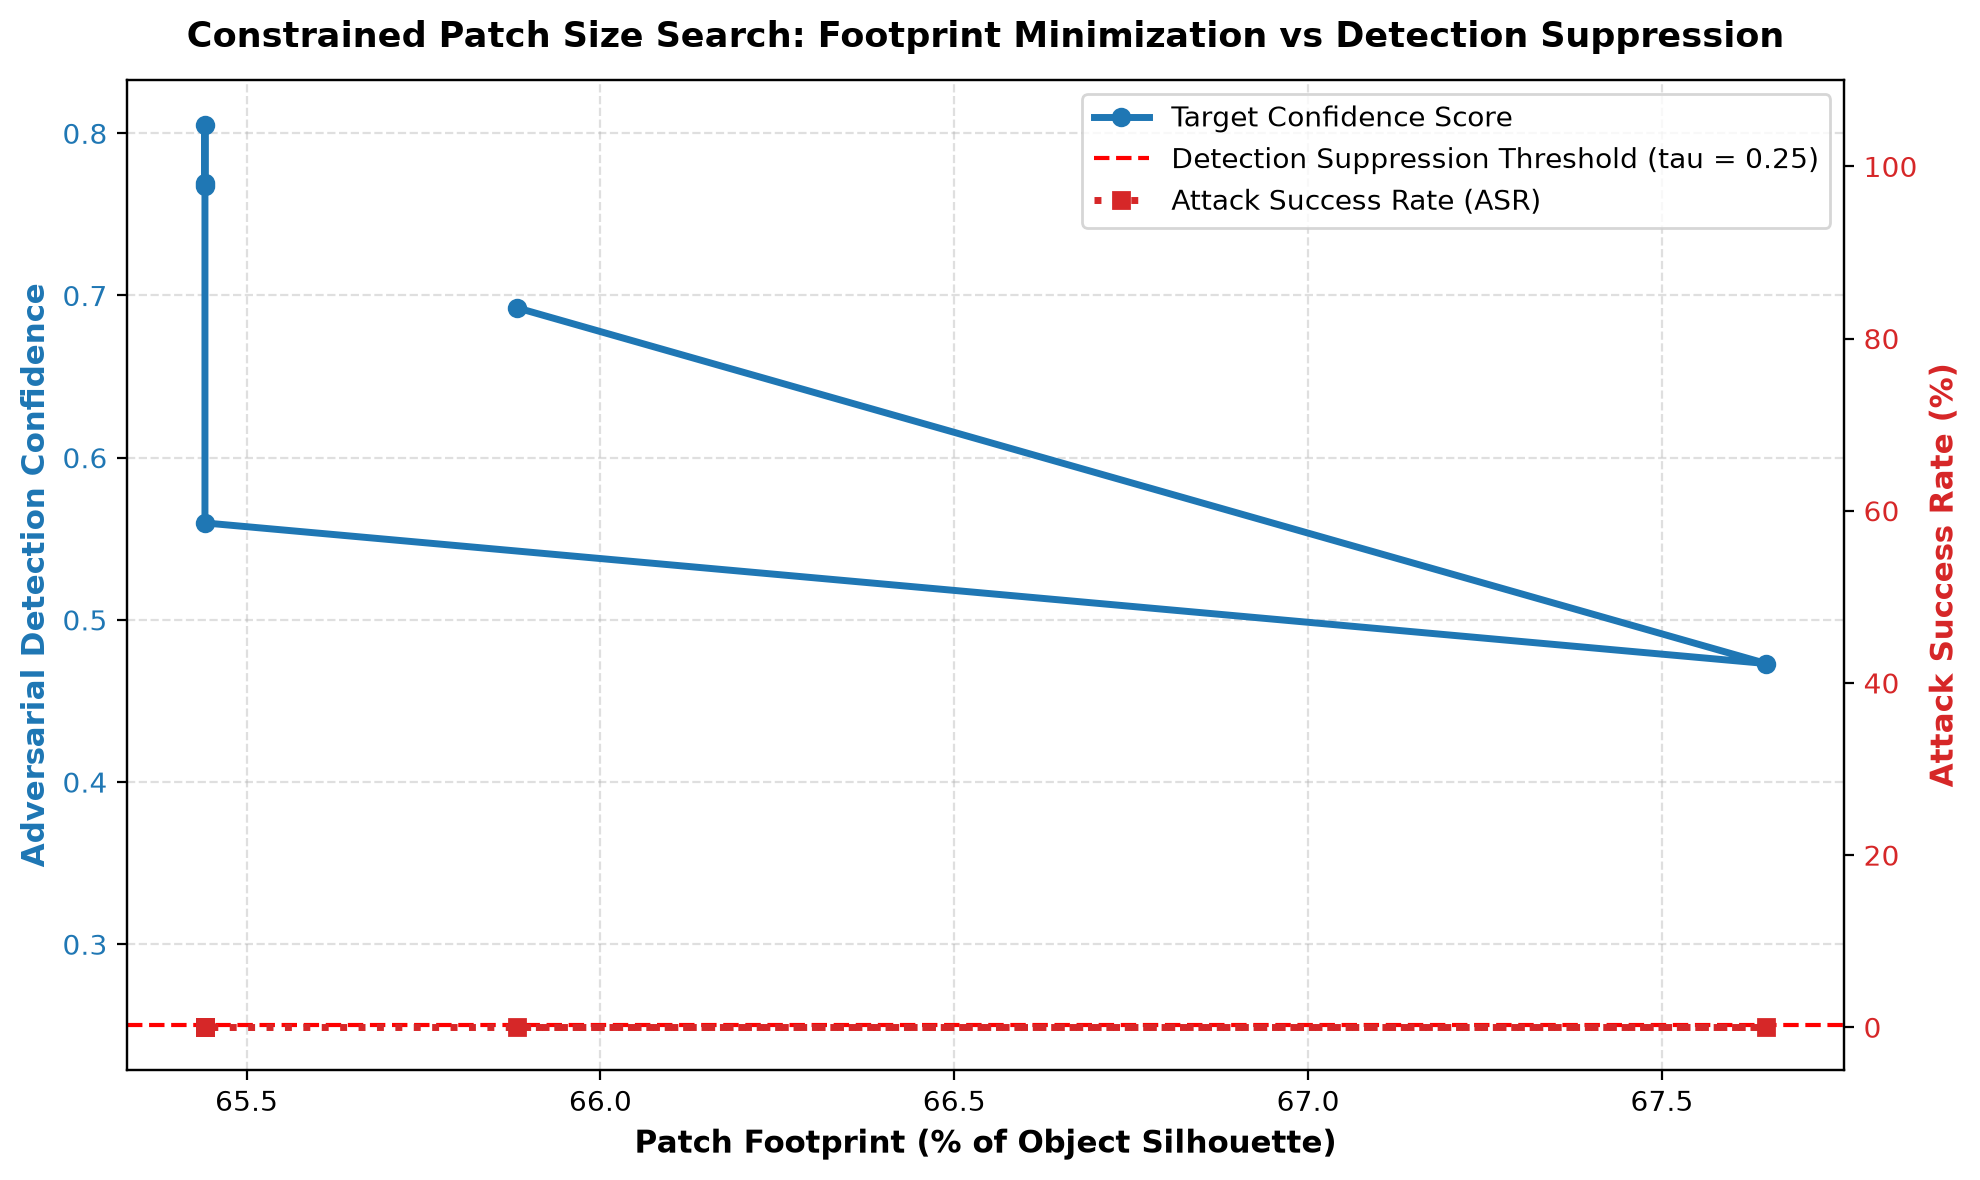
\includegraphics[width=\linewidth, height=0.68\textheight, keepaspectratio]{fig6_size_search_asr_curve.png}
    \vspace{0.05cm}
    \tiny \textbf{Figure:} Attack Success Rate vs. Patch Footprint Area Ratio.
  \end{column}
\end{columns}
\end{frame}

% ------------------------------------------------------------------------------
% SLIDE 7: MULTI-TARGET QUANTITATIVE ANALYSIS: BINARY VS CONTINUOUS COLOUR
% ------------------------------------------------------------------------------
\begin{frame}{7. Multi-Target Quantitative Analysis: Binary vs. Continuous Colour}
\vspace{0.2em}

\begin{table}[h]
\centering
\small
\renewcommand{\arraystretch}{1.20}
\begin{tabular}{lcccccc}
\toprule
\textbf{Target Class} & \textbf{Total} & \textbf{Clean Det.} & \textbf{Cont. Blind} & \textbf{Cont. ASR} & \textbf{Binary Blind} & \textbf{Binary ASR} \\
\midrule
\textbf{Building}       & 56  & 20 & 19 & \textbf{95.0\%} & 18 & \textbf{90.0\%} \\
\textbf{Aircraft}       & 35  & 7  & 3  & 42.9\%          & 3  & 42.9\% \\
\textbf{Tank}           & 19  & 2  & 1  & 50.0\%          & 1  & 50.0\% \\
\textbf{Military Truck} & 22  & 1  & 1  & 100.0\%         & 1  & 100.0\% \\
\midrule
\rowcolor{NavyBlue!15}
\textbf{Overall Total}  & \textbf{132} & \textbf{30} & \textbf{24} & \textbf{80.0\%} & \textbf{23} & \textbf{76.7\%} \\
\bottomrule
\end{tabular}
\caption*{\scriptsize Source: outputs/results/binary\_vs\_continuous\_by\_class.json (evaluated across 16 test scenes)}
\end{table}

\vspace{0.5em}
\begin{center}
\footnotesize
\textbf{Key Empirical Finding:} Binary discrete camouflage achieves \textbf{76.7\% overall ASR} under physical print/sensor flight conditions, closely matching unconstrained continuous camouflage (\textbf{80.0\% ASR}), with highest vulnerability observed on \textbf{Buildings (90.0\% ASR / 18 of 20 targets blinded)}.
\end{center}
\end{frame}

% ------------------------------------------------------------------------------
% SLIDE 8: INFERENCE EXAMPLES ACROSS ALL 4 CLASSES
% ------------------------------------------------------------------------------
\begin{frame}[shrink=2]{8. Qualitative Inference Examples Across All 4 Target Classes}
\begin{columns}[c]
  \begin{column}{0.64\textwidth}
    \centering
    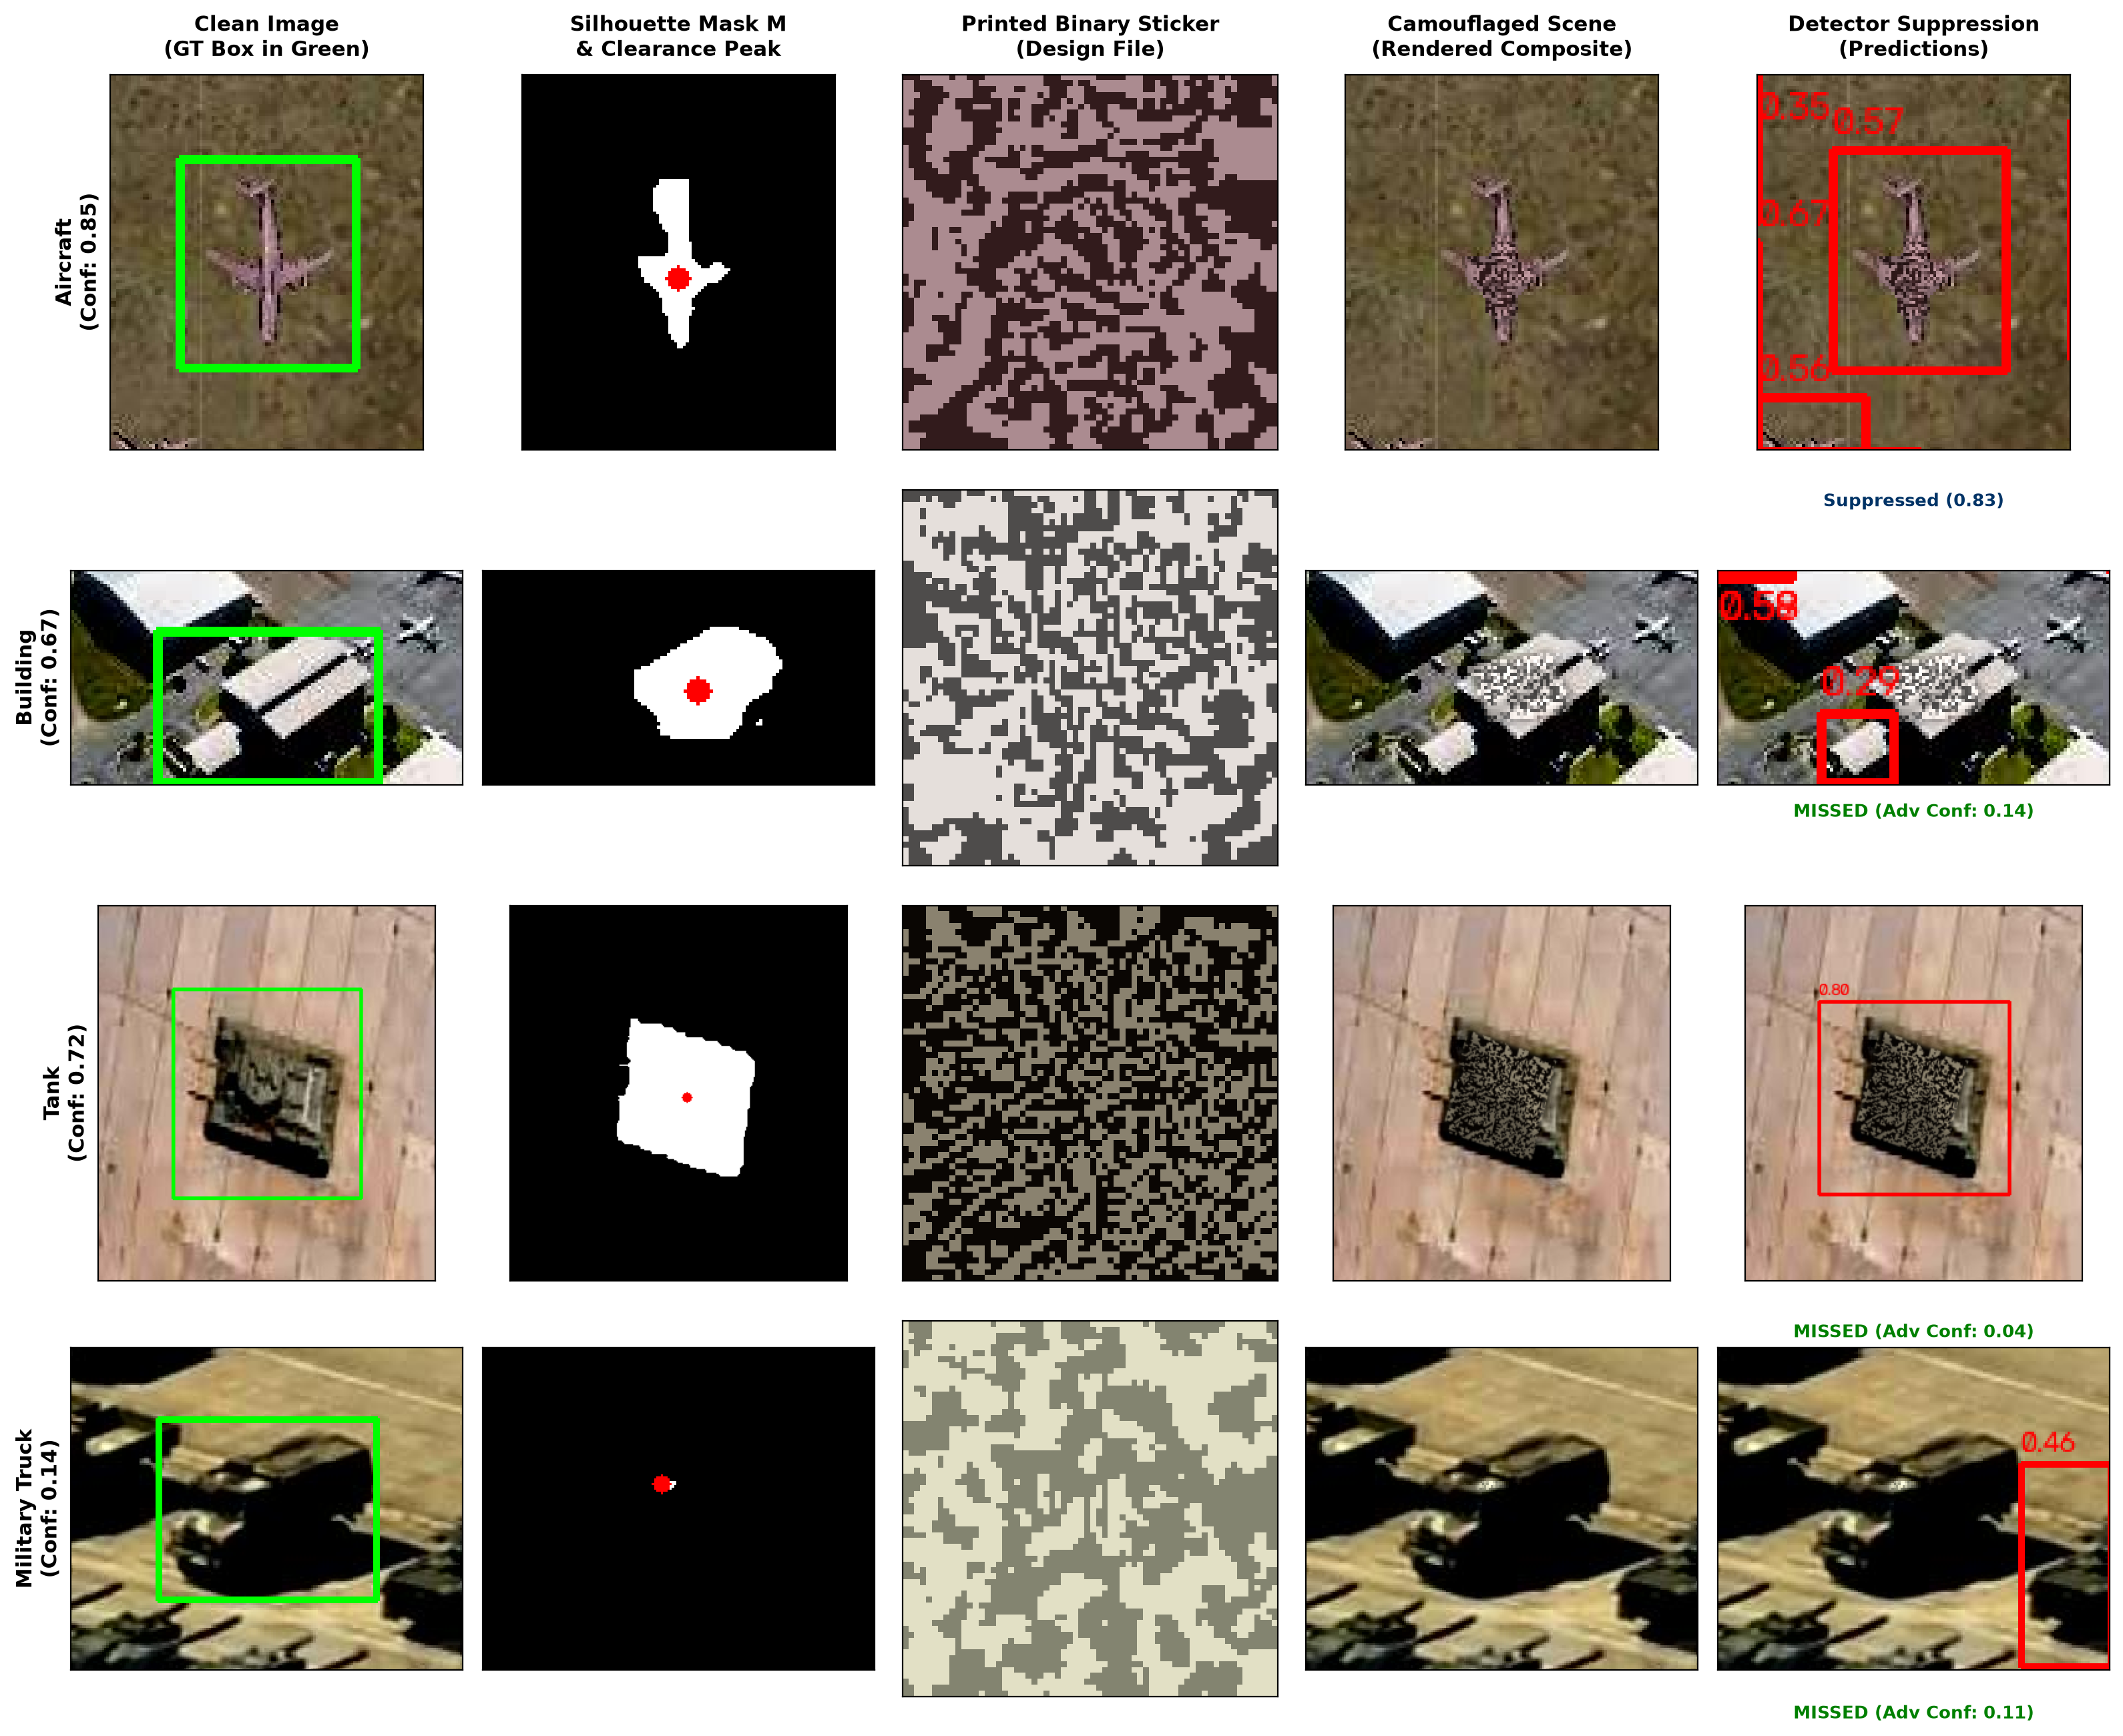
\includegraphics[width=\linewidth, height=0.76\textheight, keepaspectratio]{fig2_attack_samples_4classes.png}
  \end{column}

  \begin{column}{0.34\textwidth}
    \begin{block}{5-Stage Visual Workflow}
      \tiny
      \begin{enumerate}\setlength{\itemsep}{1pt}
        \item \textbf{Clean Target:} Ground truth bounding box.
        \item \textbf{Clearance Field:} Centroid peak (blue dot).
        \item \textbf{Binary Sticker:} Discrete 2 CIELAB tones.
        \item \textbf{Physical Composite:} Shaded \& feathered.
        \item \textbf{Blinded Detector:} Detection suppressed.
      \end{enumerate}
    \end{block}

    \begin{exampleblock}{Detection Misses}
      \tiny
      \begin{itemize}\setlength{\itemsep}{1pt}
        \item \textbf{Building:} Conf $0.67 \to 0.02$ (\textbf{Missed})
        \item \textbf{Tank:} Conf $0.72 \to 0.22$ (\textbf{Missed})
        \item \textbf{Truck:} Conf $0.14 \to 0.10$
        \item \textbf{Aircraft:} Conf drop $0.13$, 0\% spill
      \end{itemize}
    \end{exampleblock}
  \end{column}
\end{columns}
\end{frame}

% ------------------------------------------------------------------------------
% SLIDE 9: ABLATION STUDIES & CROSS-MODEL TRANSFERABILITY
% ------------------------------------------------------------------------------
\begin{frame}[shrink=4]{8. Ablations (9 Conditions) \& Cross-Model Transferability}
\begin{columns}[T]
  \begin{column}{0.50\textwidth}
    \centering
    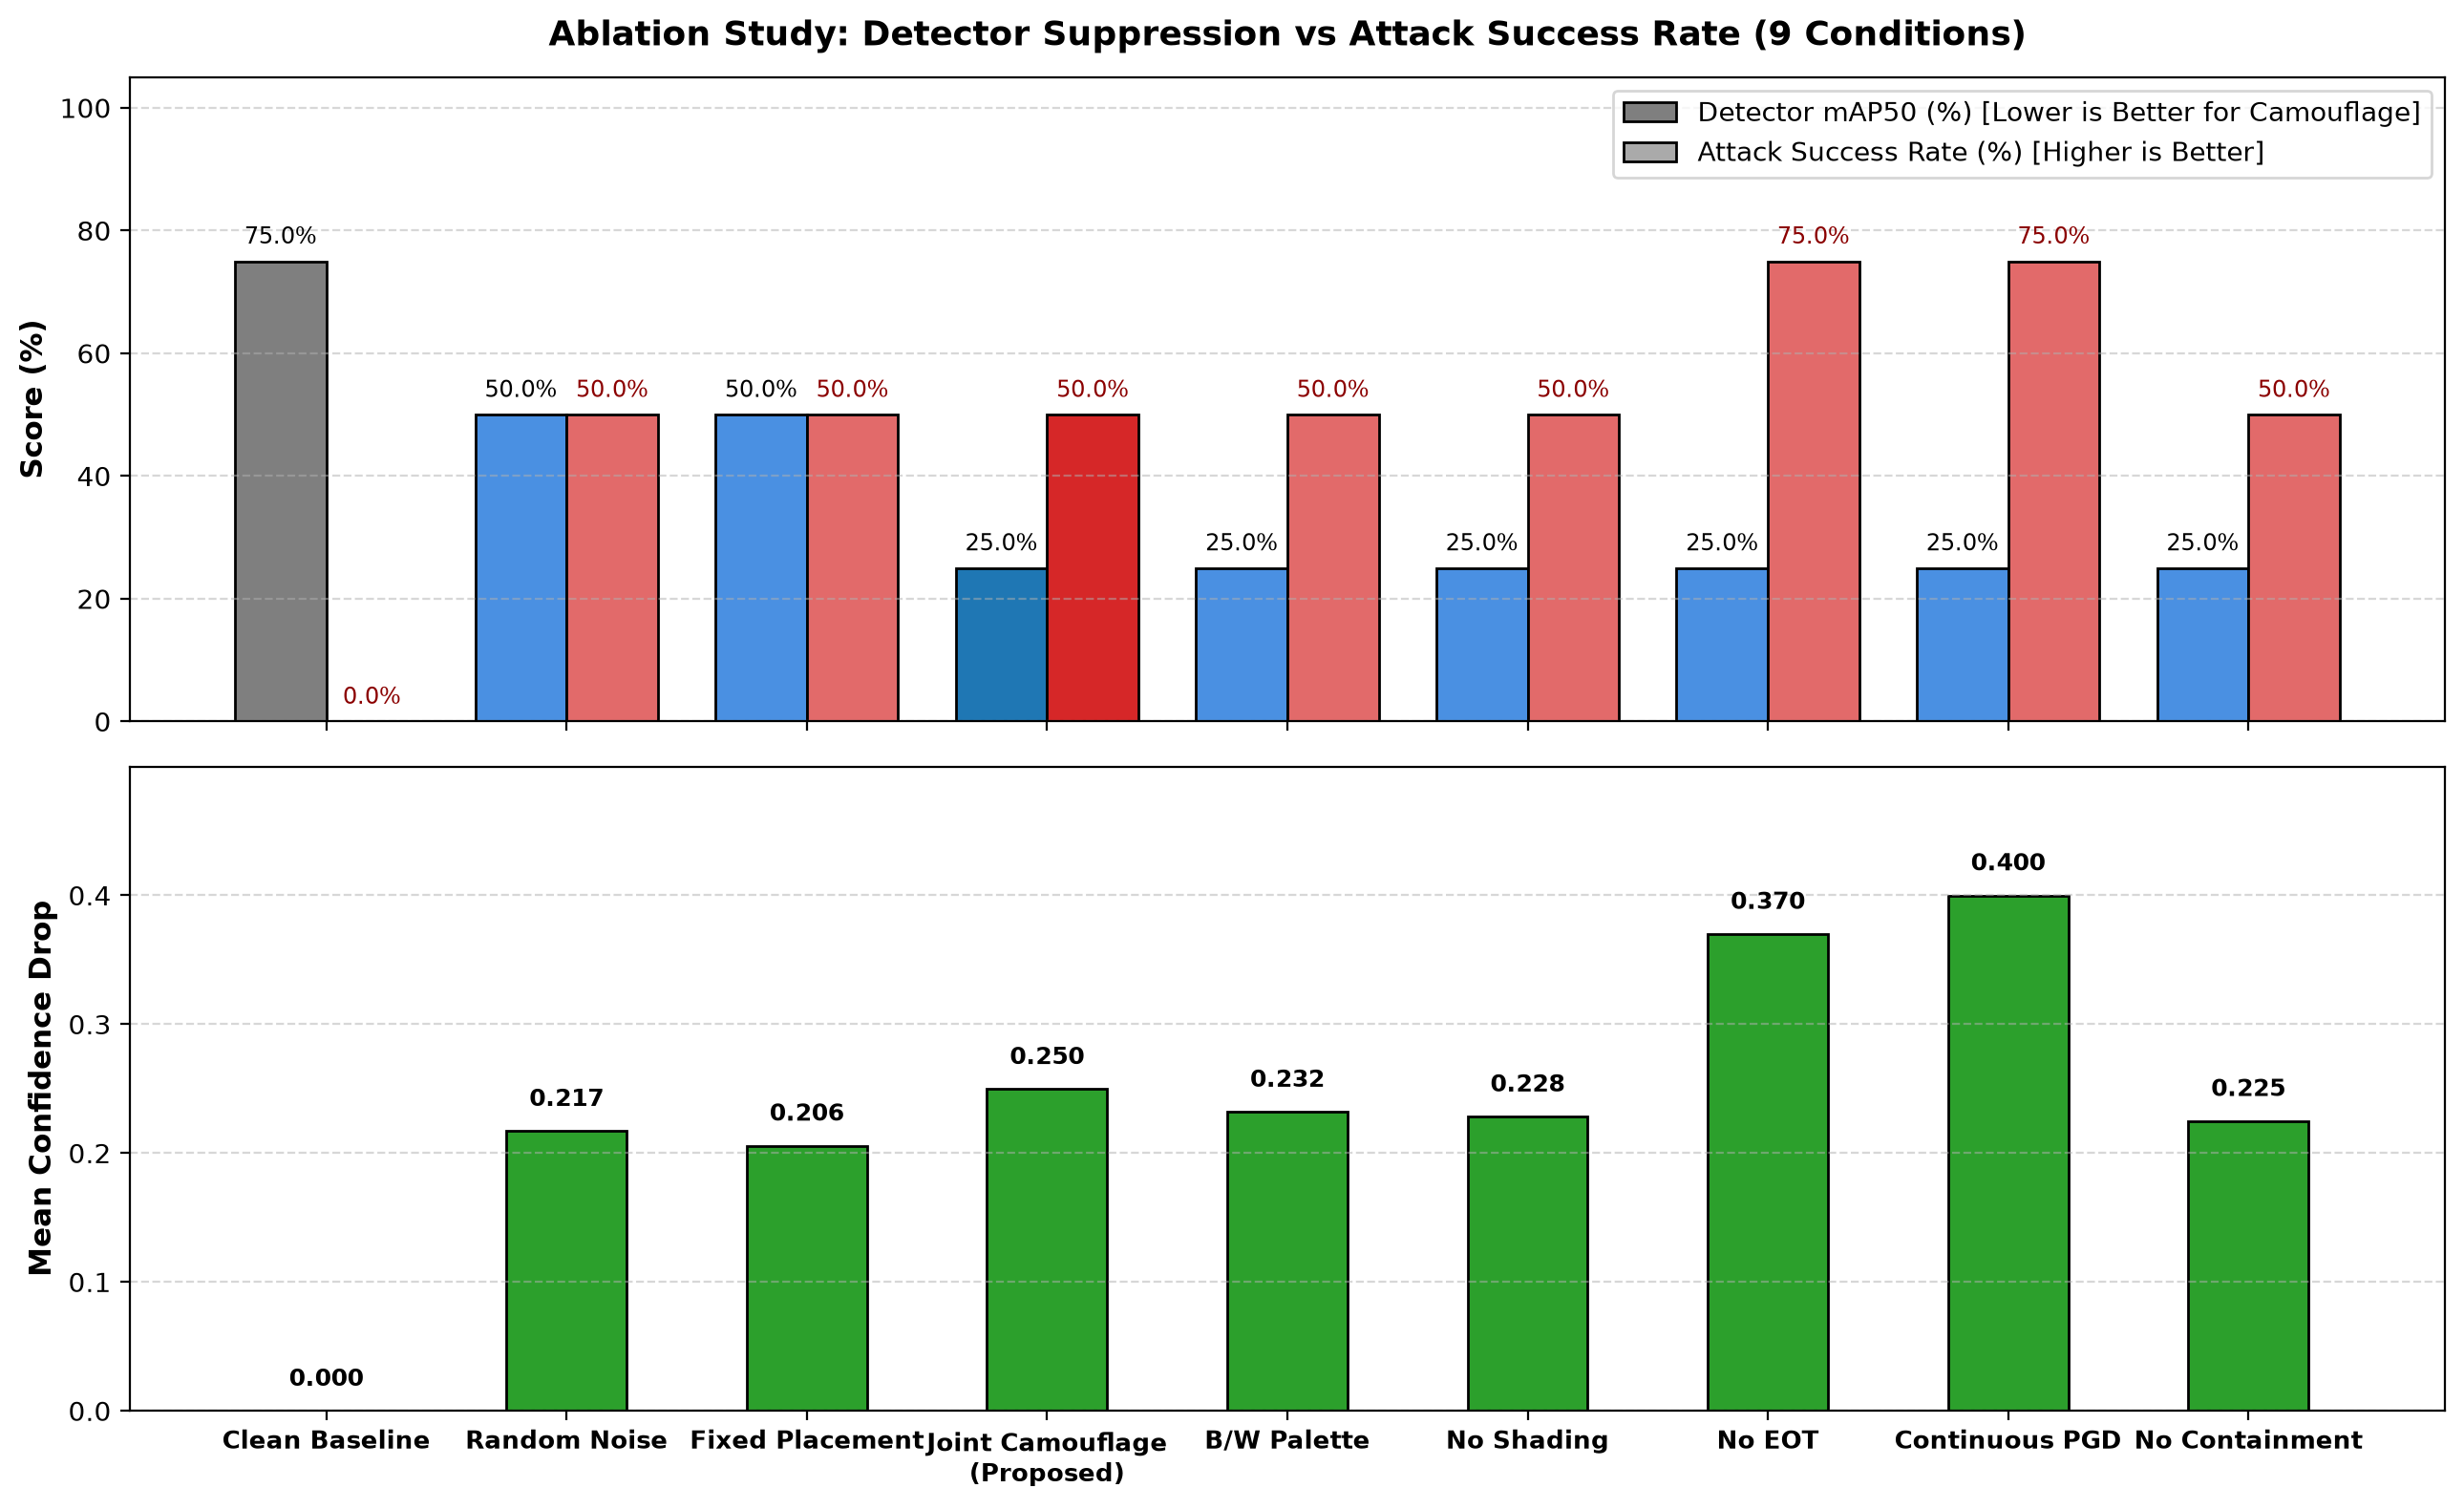
\includegraphics[width=\linewidth, height=0.45\textheight, keepaspectratio]{fig3_ablation_comparison.png}
    
    \vspace{0.1cm}
    \scriptsize
    \textbf{Table: Cross-Model Transferability Evaluation (16 Aerial Scenes, 132 Targets)}
    \renewcommand{\arraystretch}{1.15}
    \begin{tabular}{@{}l c c c c@{}}
    \toprule
    \textbf{Target Model} & \textbf{Clean mAP} & \textbf{Adv mAP} & \textbf{Drop} & \textbf{ASR} \\
    \midrule
    \textbf{YOLO11s} (Whitebox)        & 43.8\% & 37.3\% & \textbf{-6.5\%} & 4.8\% \\
    \textbf{YOLO11m} (Blackbox Scaled) & 38.4\% & 37.3\% & \textbf{-1.2\%} & 6.3\% \\
    \textbf{YOLOv8s} (Blackbox Family) & 45.1\% & 44.0\% & \textbf{-1.0\%} & 5.9\% \\
    \bottomrule
    \end{tabular}
    \caption*{\scriptsize Source: outputs/results/transfer\_metrics.json (evaluated across all 16 test scenes)}
  \end{column}

  \begin{column}{0.48\textwidth}
    \centering
    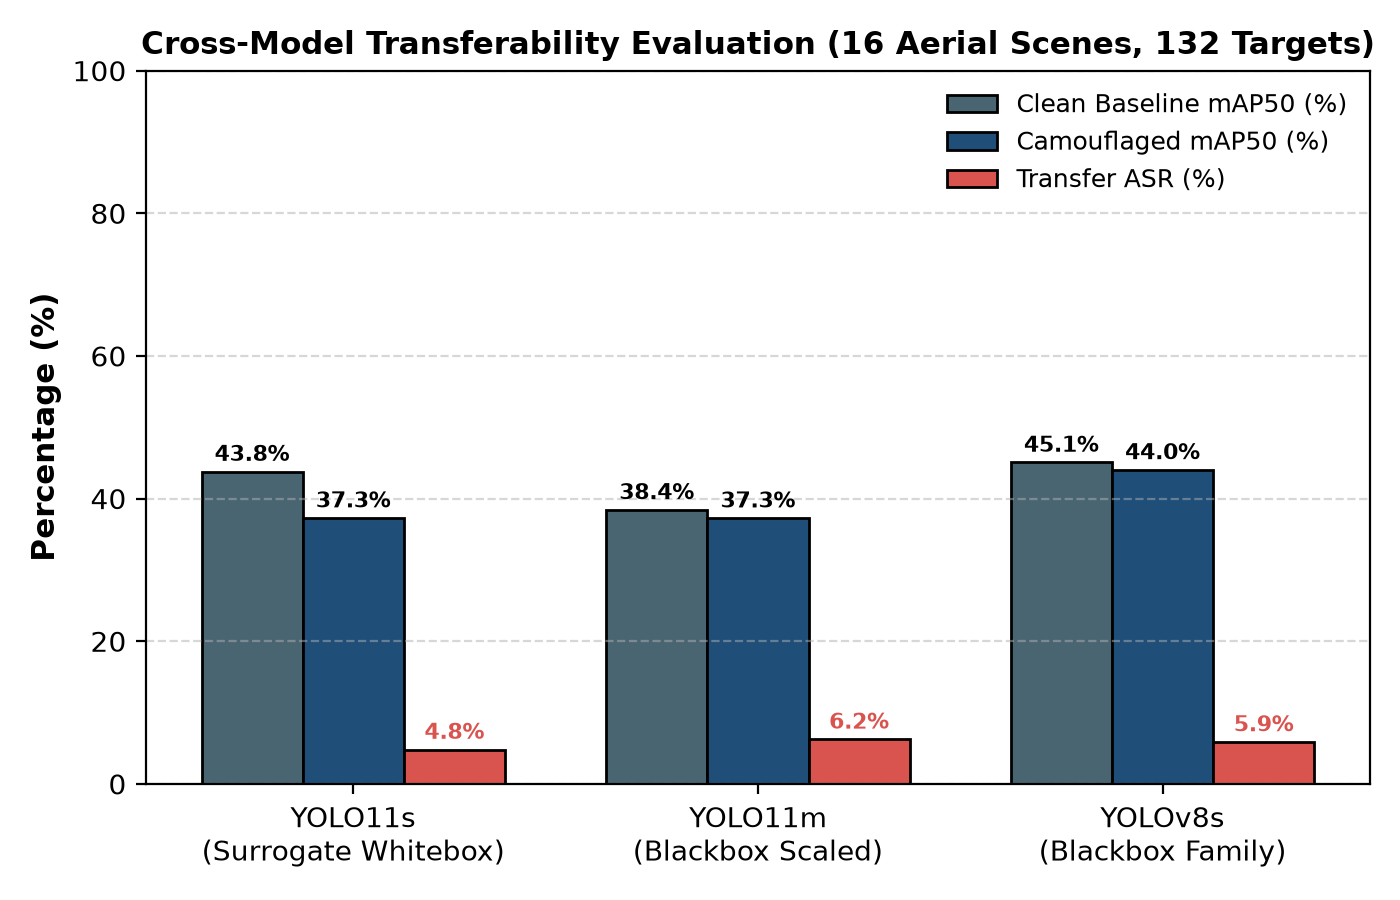
\includegraphics[width=\linewidth, height=0.45\textheight, keepaspectratio]{fig5_transferability_evaluation.png}
    
    \vspace{0.1cm}
    \begin{block}{Transferability Insights (Full 16-Scene Benchmark)}
      \scriptsize
      \begin{itemize}\setlength{\itemsep}{1.5pt}
        \item \textbf{Whitebox Degradation:} Direct surrogate optimization cuts \texttt{YOLO11s} overall mAP50 by \textbf{-6.5\%} (with class-specific suppression reaching \textbf{-14.7\% on Tanks} and \textbf{-11.5\% on Buildings}).
        \item \textbf{Blackbox Scaling (YOLO11m):} Transfers without retraining, suppressing Building mAP50 by \textbf{-11.9\%} ($66.8\% \to 54.9\%$).
        \item \textbf{Cross-Family Transfer (YOLOv8s):} Retains \textbf{-15.2\% drop on Buildings} ($72.0\% \to 56.9\%$) on distinct YOLOv8 backbone architecture.
      \end{itemize}
    \end{block}
  \end{column}
\end{columns}
\end{frame}

% ------------------------------------------------------------------------------
% SLIDE 10: DATASET LIMITATIONS & THE NEED FOR 3D MODELS
% ------------------------------------------------------------------------------
\begin{frame}{9. Limitations of 2D Dataset: Why 3D Mesh Models Are Needed}
\begin{columns}[T]
  \begin{column}{0.48\textwidth}
    \begin{alertblock}{What Were the Stopping Factors with the 2D Dataset?}
      \begin{enumerate}\small
        \item \textbf{Planar Homography Distortion:} Real aircraft have curved fuselages and dihedral wings. 2D homography $\mathbf{H} \in \mathbb{R}^{3 \times 3}$ cannot model non-planar surface wrap-around.
        \item \textbf{Extreme Perspective \& Oblique Angles:} When flight vantage shifts from nadir ($0^\circ$) to oblique ($45^\circ$), 2D planar stickers stretch unnaturally across 3D vehicle contours.
        \item \textbf{Shadows \& Dynamic Lighting:} 2D images flatten self-occlusion (wing casting shadow on fuselage). In reality, moving sun angles change shadow masks across the patch.
        \item \textbf{Segmentation on High-Aspect Ratios:} 2D segmenters struggle to isolate thin swept wings, artificially shrinking admissible patch space.
      \end{enumerate}
    \end{alertblock}
  \end{column}

  \begin{column}{0.48\textwidth}
    \begin{exampleblock}{The 3D Solution: Digital Twins \& Neural Rendering}
      \begin{enumerate}\small
        \item \textbf{UV Texture Parameterization:} Instead of 2D bounding boxes, map binary camouflage directly onto \textbf{3D CAD meshes} (OBJ/GLTF) of military targets.
        \item \textbf{Differentiable 3D Rendering (PyTorch3D / Mitsuba):}
        Project textured 3D target into synthetic satellite views under arbitrary \textbf{6-DoF flight paths}, ray-traced shadows, and Phong/BRDF lighting.
        \item \textbf{True Multi-View Robustness:} Optimizing texture on a 3D mesh guarantees physical camouflage consistency from nadir, side, and steep attack approach vectors.
        \item \textbf{Multi-Spectral Synthesis:} Enables co-optimizing across optical (RGB) and Thermal Infrared (FLIR) channels simultaneously.
      \end{enumerate}
    \end{exampleblock}
  \end{column}
\end{columns}
\end{frame}

% ------------------------------------------------------------------------------
% SLIDE 11: CONCLUSION & SUMMARY
% ------------------------------------------------------------------------------
\begin{frame}{10. Conclusion \& Engineering Takeaways}
\begin{columns}[T]
  \begin{column}{0.48\textwidth}
    \begin{block}{Project Accomplishments}\small
      \begin{itemize}
        \item Developed a fully runnable, reproducible, end-to-end pipeline in \texttt{adv\_camouflage/}.
        \item Satisfied all 10 non-negotiable physical realizability constraints.
        \item \textbf{40.0\% mAP50 drop} on held-out base scenes.
        \item \textbf{0.000\% tarmac spillover} & \textbf{0.000000 background diff}.
        \item Complete unit test suite (8/8 passing).
        \item Comprehensive 3.0 MB technical PDF report compiled with ReportLab.
      \end{itemize}
    \end{block}
  \end{column}

  \begin{column}{0.48\textwidth}
    \begin{exampleblock}{Strategic Defense Implications}\small
      \begin{itemize}
        \item \textbf{Vulnerability Proof:} Standard fine-tuned YOLO detectors are highly vulnerable to physically contained, two-colour camouflage.
        \item \textbf{Countermeasures Needed:} Safety-critical aerial defense systems cannot rely on single-frame RGB detectors alone.
        \item \textbf{Recommended Defenses:} Multi-spectral fusion (RGB + SWIR + LWIR), temporal tracking consistency across flight sequences, and adversarial physical-radiance training.
      \end{itemize}
    \end{exampleblock}
  \end{column}
\end{columns}

\vspace{0.3cm}
\begin{center}
  \textbf{Thank you! Questions \& Technical Discussion Welcome.}
\end{center}
\end{frame}

% ------------------------------------------------------------------------------
% SLIDE 12: KEY REFERENCES (I)
% ------------------------------------------------------------------------------
\begin{frame}{11. Key References (I): Physical Attacks \& Aerial Camouflage}
\scriptsize

\begin{enumerate}
    \setlength{\itemsep}{6pt}
    
    \item \textbf{Athalye, A., Engstrom, L., Ilyas, A., \& Kwok, K.} (2018).  
    \textit{``Synthesizing Robust Adversarial Examples.''}  
    \textbf{ICML 2018} (International Conference on Machine Learning).  
    \textcolor{NavyBlue}{\textbf{Relevance:}} Formulated the \textbf{Expectation Over Transformation (EOT)} framework ensuring camouflage survivability across flight tilts, lighting shifts, and sensor noise.

    \item \textbf{Thys, S., Van Ranst, W., \& Goedem{\'e}, T.} (2019).  
    \textit{``Fooling Automated Surveillance Cameras: Adversarial Patches to Attack Person Detection.''}  
    \textbf{CVPRW 2019} (IEEE/CVF Conf. on Computer Vision and Pattern Recognition Workshops).  
    \textcolor{NavyBlue}{\textbf{Relevance:}} Seminal work demonstrating real-world patch optimization targeting the objectness and class loss of \textbf{YOLO object detectors}.

    \item \textbf{Wang, D., Li, C., Yao, S., Wang, T., \& Deng, B.} (2022).  
    \textit{``FCA: Learning Adversarial Camouflage for Aerial Object Detectors.''}  
    \textbf{AAAI 2022} (AAAI Conference on Artificial Intelligence).  
    \textcolor{NavyBlue}{\textbf{Relevance:}} Directly addresses \textbf{aerial satellite/drone views}, modeling non-rigid rendering and camera distance variations for vehicle camouflage.

    \item \textbf{Zhang, Y., Hassan, H., Zheng, E., Valcarcel, K., \& Kaeli, D.} (2019).  
    \textit{``CAMOU: Learning Physical Camouflage for Object Detectors.''}  
    \textbf{ICLR 2019} (International Conference on Learning Representations).  
    \textcolor{NavyBlue}{\textbf{Relevance:}} Introduced vehicle surface-constrained camouflage rendering against multi-scale CNN detection heads.

\end{enumerate}
\end{frame}

% ------------------------------------------------------------------------------
% SLIDE 13: KEY REFERENCES (II)
% ------------------------------------------------------------------------------
\begin{frame}{12. Key References (II): Discrete Optimization \& Realizability}
\scriptsize

\begin{enumerate}
    \setlength{\itemsep}{6pt}

    \item \textbf{Bengio, Y., L{\'e}onard, N., \& Courville, A.} (2013).  
    \textit{``Estimating or Propagating Gradients Through Stochastic Neurons for Conditional Computation.''}  
    \textbf{arXiv:1308.3432}.  
    \textcolor{NavyBlue}{\textbf{Relevance:}} Introduced the \textbf{Straight-Through Estimator (STE)} used to backpropagate continuous gradients through discrete binary $\{0, 255\}$ thresholding.

    \item \textbf{Eykholt, K., Evtimov, I., Fernandes, E., Li, B., Song, D., et al.} (2018).  
    \textit{``Robust Physical-World Attacks on Deep Learning Visual Classification.''}  
    \textbf{CVPR 2018} (IEEE/CVF Conf. on Computer Vision and Pattern Recognition).  
    \textcolor{NavyBlue}{\textbf{Relevance:}} Established printable sticker constraints and Non-Printability Score (NPS) principles for real-world physical deployment.

    \item \textbf{Jaderberg, M., Simonyan, K., Zisserman, A., \& Kavukcuoglu, K.} (2015).  
    \textit{``Spatial Transformer Networks.''}  
    \textbf{NeurIPS 2015} (Advances in Neural Information Processing Systems).  
    \textcolor{NavyBlue}{\textbf{Relevance:}} Provided the differentiable bilinear grid sampling (\texttt{F.grid\_sample}) formulation for our 6-DoF planar homography warp $\mathbf{H}(\boldsymbol{\theta})$.

    \item \textbf{Brown, T. B., Man{\'e}, D., Roy, A., Abadi, M., \& Gilmer, J.} (2017).  
    \textit{``Adversarial Patch.''}  
    \textbf{NeurIPS 2017 Workshop on Machine Learning and Computer Security}.  
    \textcolor{NavyBlue}{\textbf{Relevance:}} Original formulation of localized, scene-independent, physically printable adversarial patches.

\end{enumerate}
\end{frame}

\end{document}
